% Options for packages loaded elsewhere
\PassOptionsToPackage{unicode}{hyperref}
\PassOptionsToPackage{hyphens}{url}
%
\documentclass[
]{article}
\usepackage{lmodern}
\usepackage{amssymb,amsmath}
\usepackage{ifxetex,ifluatex}
\ifnum 0\ifxetex 1\fi\ifluatex 1\fi=0 % if pdftex
  \usepackage[T1]{fontenc}
  \usepackage[utf8]{inputenc}
  \usepackage{textcomp} % provide euro and other symbols
\else % if luatex or xetex
  \usepackage{unicode-math}
  \defaultfontfeatures{Scale=MatchLowercase}
  \defaultfontfeatures[\rmfamily]{Ligatures=TeX,Scale=1}
\fi
% Use upquote if available, for straight quotes in verbatim environments
\IfFileExists{upquote.sty}{\usepackage{upquote}}{}
\IfFileExists{microtype.sty}{% use microtype if available
  \usepackage[]{microtype}
  \UseMicrotypeSet[protrusion]{basicmath} % disable protrusion for tt fonts
}{}
\makeatletter
\@ifundefined{KOMAClassName}{% if non-KOMA class
  \IfFileExists{parskip.sty}{%
    \usepackage{parskip}
  }{% else
    \setlength{\parindent}{0pt}
    \setlength{\parskip}{6pt plus 2pt minus 1pt}}
}{% if KOMA class
  \KOMAoptions{parskip=half}}
\makeatother
\usepackage{xcolor}
\IfFileExists{xurl.sty}{\usepackage{xurl}}{} % add URL line breaks if available
\IfFileExists{bookmark.sty}{\usepackage{bookmark}}{\usepackage{hyperref}}
\hypersetup{
  pdftitle={Propagating Sequence Uncertainty into Downstream Analyses},
  pdfauthor={David Champredon, Devan Becker, Art Poon, Connor Chato},
  hidelinks,
  pdfcreator={LaTeX via pandoc}}
\urlstyle{same} % disable monospaced font for URLs
\usepackage[margin=1in]{geometry}
\usepackage{graphicx}
\makeatletter
\def\maxwidth{\ifdim\Gin@nat@width>\linewidth\linewidth\else\Gin@nat@width\fi}
\def\maxheight{\ifdim\Gin@nat@height>\textheight\textheight\else\Gin@nat@height\fi}
\makeatother
% Scale images if necessary, so that they will not overflow the page
% margins by default, and it is still possible to overwrite the defaults
% using explicit options in \includegraphics[width, height, ...]{}
\setkeys{Gin}{width=\maxwidth,height=\maxheight,keepaspectratio}
% Set default figure placement to htbp
\makeatletter
\def\fps@figure{htbp}
\makeatother
\setlength{\emergencystretch}{3em} % prevent overfull lines
\providecommand{\tightlist}{%
  \setlength{\itemsep}{0pt}\setlength{\parskip}{0pt}}
\setcounter{secnumdepth}{5}



% ==== GENERAL ====

\newcommand{\warning}[1]{\textbf{\textcolor{orange}{((#1))}}}
\newcommand{\comment}[1]{\textsl{\textcolor{cyan}{((#1))}}}
\newcommand{\eg}{\textit{e.g.,}\xspace}
\newcommand{\ie}{\textit{i.e.},\xspace}

% ==== SPECIFIC ====

\newcommand{\sq}[1]{\texttt{\textcolor{brown}{#1}}}

\newcommand{\sps}{\mathcal{B}} % sequence probability sequence
\newcommand{\nps}{\mathcal{S}} % nucleotide probability sequence
\newcommand{\nlps}{nucleotide-level probabilistic sequence\xspace}
\newcommand{\slps}{sequence-level probabilistic sequence\xspace}

\newcommand{\pr}[1]{\mathbb{P}(#1)}

\newcommand{\md}{\mathcal{M}} % Multinomial distribution
\newcommand{\pois}[1]{\mathrm{Poisson}\left(#1\right)}
\newcommand{\betadist}[1]{\mathrm{Beta}\left(#1\right)}


\usepackage{xspace}
\usepackage{xcolor}
\usepackage{float}
\usepackage[]{natbib}
\bibliographystyle{plainnat}

\title{Propagating Sequence Uncertainty into Downstream Analyses}
\author{David Champredon, Devan Becker, Art Poon, Connor Chato}
\date{}

\begin{document}
\maketitle
\begin{abstract}
Genetic sequencing is subject to many different types of errors, but
most analyses treat the resultant sequences as if they are perfect.
Since the process of sequencing is very difficult, modern machines rely
on significantly larger numbers of reads rather than making each read
significantly more accurate. Still, the coverage of such machines is
imperfect and leaves uncertainty in many of the base calls. Furthermore,
there are circumstances around the sequencing that can induce further
problems. In this work, we demonstrate that the uncertainty in
sequencing techniques will affect downstream analysis and propose a
straightforward (if computationally expensive) method to propagate the
uncertainty.\\
Our method uses a probabilistic matrix representation of individual
sequences which incorporates base quality scores and makes various
uncertainty propagation methods obvious and easy. With the matrix
representation, resampling possible base calls according to quality
scores provides a bootstrap- or prior distribution-like first step
towards genetic analysis. Analyses based on these re-sampled sequences
will include an honest evaluation of the error involved in such
analyses.\\
We demonstrate our resampling method on HIV and SARS-CoV-2 data. The
resampling procedures adds computational cost to the analyses, but the
large impact on the variance in downstream estimates makes it clear that
ignoring this uncertainty leads to invalid conclusions. For HIV data, we
show that phylogenetic reconstructions are much more sensitive to
sequence error uncertainty than previously believed, and for SARS-CoV-2
data we show that lineage designations via Pangolin are much less
certain than the bootstrap support would imply.
\end{abstract}

TODO

\begin{itemize}
\tightlist
\item
  Ensure I'm using pangolin/pangoLEARN in proper contexts

  \begin{itemize}
  \tightlist
  \item
    Right now, I'm using them as synonyms (bad)
  \end{itemize}
\item
  Nomenclature:

  \begin{itemize}
  \tightlist
  \item
    \(\nps\) is ``nucleotide-level uncertainty sequence'' or simply
    ``uncertainty matrix''?

    \begin{itemize}
    \tightlist
    \item
      ``Uncertainty matrix'' is a misnomer - the entries are the
      probabilitity of basis call. Is there a better term?
    \item
      Maybe ``Call Probability Matrix''?
    \end{itemize}
  \item
    Nucleotide ``position'', ``location'', or ``locus''?
  \item
    ``sequence-level uncertainty sequence'' or ``genome likelihood''?

    \begin{itemize}
    \tightlist
    \item
      Genome likelihood is used in other contexts; their formulations
      are model-based but have the same interpretation.
    \end{itemize}
  \end{itemize}
\item
  Notation:

  \begin{itemize}
  \tightlist
  \item
    subscript \(j\) for arbitrary locations on the genome.
  \end{itemize}
\item
  Style:

  \begin{itemize}
  \tightlist
  \item
    Ensure I use \(\ie\), not i.e.
  \item
    I'm really bad at tense.
  \end{itemize}
\end{itemize}

\hypertarget{intro}{%
\section{Intro}\label{intro}}

Extracting DNA/RNA from biological samples is a complex process that
involves many steps: extraction of the genetic material of interest
(avoiding contamination with foreign/unwanted genetic material); reverse
transcription (if RNA); DNA fragmentation of the genome into smaller
segments; amplification of the fragmented sequences using PCR;
sequencing the fragments (\eg with fluorescent techniques); putting back
the small fragments together by aligning them (de novo) or mapping them
to benchmark libraries. Errors can be introduced at each of these steps
for various reasons
\citep[\citet{oraweAccountingUncertaintyDNA2015}]{beerenwinkelUltradeepSequencingAnalysis2011}
and some errors can be quantified (\eg sequencing quality scores from
chromatographs).

When the phylogenic tree to infer is based on pathogen sequences
infecting hosts, the potential genetic diversity of the infection adds a
complexity in phylogeny reconstruction. Typical examples are
epidemiological studies reconstructing transmission trees from viral
genetic sequences (\eg HIV, HepC) sampled from infected patients.

The different sources of uncertainty described above impact our
observations of the actual genetic sequences. There are standard
approaches to deal with identifiable observation errors. Base calls that
are ambiguous (from equivocal chromatograph curves or because of genuine
polymorphisms) are assigned ambiguity codes (\eg Y for C or T, R for A
or G, etc.). Alignment methods are heuristic methods based on similarity
scores that generally do not quantify the uncertainty of alignment.
Methods to reconstruct phylogenies usually leave out the uncertainty
complexity and settle for sequences composed of the most frequent
nucleotides and/or ignore ambiguity codes (with some exceptions,
e.g.~\citet{depristoFrameworkVariationDiscovery2011}).

In 1998, \citet{ewingBaseCallingAutomatedSequencer1998} and
\citet{richterichEstimationErrorsRaw1998} both showed that estimates of
the base call quality (called Phred scores) can be an accurate estimate
of the number of errors that the machines at the time would make. Modern
machines still report these Phred scores, but methods for
adjusting/recalibrating these scores for greater accuracy have been
proposed \citep[\citet{depristoFrameworkVariationDiscovery2011},
\citet{liSNPDetectionMassively2009}]{liAdjustQualityScores2004} For most
analyses, these scores are used to censor the base calls (i.e., label
them ``N'' rather than A, T, C, or G) if the base call error probability
is too high or there are too few reads and a given location. It is
commonplace to remove the sequence from analysis if the total sequence
error probability is too high \citep[see,
e.g.,][\citet{robaskyRoleReplicatesError2014},
\citet{oraweAccountingUncertaintyDNA2015}]{doroninaPhylogeneticPositionEmended2005}.
The error probability is deemed too high based on a strict threshold
(e.g.~1\% chance of error), but these thresholds aren't necessarily
standard across studies.

Some studies have incorporated the error probabilities using genome
likelihoods. \citet{depristoFrameworkVariationDiscovery2011} and
\citet{gompertHierarchicalBayesianModel2011} incoporate the adjusted
Phred scores into a likelihood framework that allows them to more
accurately estimate population-level allele distributions.
\citet{fumagalliQuantifyingPopulationGenetic2013a} present a new
estimator for population genetic diversity based on such analyses.
\citet{kuoEAGLEExplicitAlternative2018} use genome likelihoods to
perform hypothesis tests that evaluate whether a given genome sequence
is consistent with a given alternative sequence, after accounting for
the errors. As with any parametric model-based approach, genome
likelihoods use assumptions about the errors in order to make
conclusions about the underlying patterns.

Few other authors have considered the uncertainty present in the
sequences in downstream analyses. One notable exception is
\citet{oraweAccountingUncertaintyDNA2015}, who suggest methods for
propagating sequence-level uncertainty into determining whether two
subjects have the same alleles as well as incorporating the
sequence-level uncertainty into confidence intervals for allele
frequency.

In our work, we present a simple, general framework that can be
incorporated into any analysis of genetic sequence data. This framework
involves converting the uncertainty scores into a matrix of
probabilities, and repeatedly sampling from this matrix and using the
resultant samples in downstream analysis. Unlike likelihood-based
approaches, we do not make assumptions about the underlying patterns in
the data. In doing so, we gain generalizability at the expense of
computation time. Our technique is amenable to any appropriate quality
score adjustments prior to building the uncertainty matrix.

\hypertarget{methods}{%
\section{Methods}\label{methods}}

\hypertarget{probabilistic-representation-of-sequences}{%
\subsection{Probabilistic Representation of
Sequences}\label{probabilistic-representation-of-sequences}}

Here, we describe two theoretical frameworks to model sequence
uncertainty at the \emph{nucleotide level} or at the
\emph{sequence level}. In both frameworks, the sequence of nucleotides
from a biological sample is not treated as a certain observation, but
rather as a collection of possible sequences.

\hypertarget{nucleotide-level-uncertainty}{%
\subsubsection{Nucleotide-level
uncertainty}\label{nucleotide-level-uncertainty}}

To represent the uncertainty at each location along the genome, we
introduce following matrix:

\begin{equation}
\nps = \bordermatrix{   & 1 & 2 & \ldots & \ell \cr
                \sq{A} & \nps_{A, 1} & \nps_{A, 2} & \ldots & \nps_{A, \ell} \cr
                \sq{C} & \nps_{C, 1} & \nps_{C, 2} & \ldots & \nps_{C, \ell} \cr
                \sq{G} & \nps_{G, 1} & \nps_{G, 2} & \ldots & \nps_{G, \ell} \cr
                \sq{T} & \nps_{T, 1} & \nps_{T, 2} & \ldots & \nps_{T, \ell} \cr 
                \sq{-} & \nps_{x, 1} & \nps_{x, 2} & \ldots & \nps_{x, \ell} \cr 
}\label{eq:nps}
\end{equation}

Each column represents the nucleotide position, each row one of the four
nucleotide \sq{A,C,G,T} as well as an empty position ``\sq{-}''" that
symbolizes a genuine deletion (not caused by missing data). Hence,
\(\nps\) is a \(5\times\ell\) matrix. Its elements represent the
probability that a nucleotide is at given position:

\begin{equation}
\nps_{\sq{n},j} = \pr{\text{nucleotide \sq{n} is at position }j}
\end{equation} with the special case for a deletion:

\begin{equation}
\nps_{\sq{-},j} = \pr{\text{empty position }j}
\end{equation} Note that we have for all \(1\leq j \leq \ell\):
\begin{equation}
\sum_{n\in \{ \sq{A,C,G,T,-} \} } \nps_{n, j} = 1
\end{equation} Also, the sequence length is stochastic if
\(\nps_{\sq{-},i}>0\) for at least one \(i\). The probability that the
sequence has the maximum length \(\ell\) is
\(\prod_{i=1}^\ell (1-\nps_{\sq{-},i})\). We call the matrix \(\nps\)
the \emph{\nlps} of a biological sample. The nucleotide (or deletion)
drawn at each position is independent from all the others, so there are
\(5^\ell\) possible different sequences for a given probabilistic
nucleotide sequence, but these sequences are \emph{not} equally
probable.

\hypertarget{sequence-level-uncertainty}{%
\subsubsection{Sequence-level
uncertainty}\label{sequence-level-uncertainty}}

Out of the \(5^\ell\) possible sequences, the nucleotide uncertainty may
assign a positive probability to sequences that are not biologically
possible. As an alternative representation and to reduce the space of
possible sequences, let's assume we have enough information (either
directly observed from data or simulated) to generate a set of sequences
\(\sps = (\sps_i)_{i\in\{1\ldots m\} }\) of all \(m\) biologically
possible sequences. Note that the \(\sps_i\) do not have necessarily the
same length. The observed genetic sequence, \(s\), is a sample from a
specified distribution \(a\): \begin{equation}
\pr{s = \sps_i} = a(i)
\end{equation} We call the set \(\sps\) the \emph{\slps}. Note that,
because \(a\) is a distribution, we must have \(\sum_{i=1}^m a(i) = 1\).

If we have the following \nlps: \[
\nps = 
\bordermatrix{
& \scriptscriptstyle{1} & \scriptscriptstyle{2}& \scriptscriptstyle{3}& \scriptscriptstyle{4} & \scriptscriptstyle{5} & \scriptscriptstyle{6} \cr
\sq{A} & 0.9 & 0.05   & 0.99 & 0 & 0 & 0.6\cr
\sq{C} & 0   & 0.8 & 0 & 0 & 0.1 & 0.1\cr
\sq{G} & 0.1 & 0.15 & 0 & 0.3 & 0.9 & 0\cr
\sq{T} & 0 & 0 & 0.01 & 0.7 & 0 & 0.3\cr
\sq{-} & 0 & 0 & 0 & 0 & 0 & 0\cr
}
\] then there are \(2\times 3 \times 2^3 \times 3 = 144\) possible
sequences. The most likely is the one having the highest nucleotides
probabilities: \sq{ACATGA} with probability 0.2694
(\(0.9\times 0.8\times 0.99 \times 0.7 \times 0.9 \times 0.6\)).

If there is a positive probability of deletion for at least one
position, then the sequence has a variable length. Let's take the same
example as above, but adding one possible empty position:

\[
\nps = 
\bordermatrix{
&\scriptscriptstyle{1} & \scriptscriptstyle{2}& \scriptscriptstyle{3}& \scriptscriptstyle{4} & \scriptscriptstyle{5} & \scriptscriptstyle{6} \cr
\sq{A} & 0.9 & 0.05   & 0.99 & 0 & 0 & 0.6\cr
\sq{C} & 0   & 0.8 & 0 & 0 & 0.1 & 0.1\cr
\sq{G} & 0.1 & 0.15 & 0 & 0.2 & 0.9 & 0\cr
\sq{T} & 0 & 0 & 0.01 & 0.7 & 0 & 0.3\cr
\sq{-} & 0 & 0 & 0 & 0.1 & 0 & 0\cr
}
\]

\noindent Like above, there is still a 0.2694 probability that the
sequence is \sq{ACATGA}, but now there is a chance that position 4 is
deleted. For example, with probability 0.038 the sequence is
\sq{ACA-GA}.

Below is an example for a \slps \(\sps\):

\begin{table}[H]
\begin{center}
\begin{tabular}{lc}
\hline
\textbf{sequence} & $a$ \\
\hline
\sq{ACATGA} & 0.60 \\
\sq{ACATCA} & 0.12 \\
\sq{AGATCA} & 0.15 \\
\sq{ACAGA}  & 0.05 \\
\sq{GCATGA} & 0.08 \\
\hline
\end{tabular}
\end{center}
\label{default}
\end{table}

\% Sampling from \(\sps\), we will have for example \sq{ACATCA} \(12\%\)
of the time. Large genomes, such as SARS-CoV-2, will result in vanishly
small probabilities for all sequences, and thus work on the log scale is
often preferred.

\hypertarget{deletions-and-insertions}{%
\subsection{Deletions and Insertions}\label{deletions-and-insertions}}

By construction, the \nlps must be defined with its longest possible
length. Deletions are naturally modelled with our representation but
insertions have to be modelled using deletion probability.

Consider the following \nlps: \begin{equation}
\label{eq:indel}
\nps = 
\bordermatrix{
&\scriptscriptstyle{1} & \scriptscriptstyle{2}& \scriptscriptstyle{3}& \scriptscriptstyle{4} & \scriptscriptstyle{5} & \scriptscriptstyle{6} \cr
\sq{A} & 0 & 0   & 1 & 0    & 1 & 0\cr
\sq{C} & 1 & 0    & 0 & 0    & 0 & 0\cr
\sq{G} & 0 & 0.99 & 0 & 0    & 0 & 0\cr
\sq{T} & 0 & 0    & 0 & 0.01 & 0 & 1\cr
\sq{-} & 0 & 0.01 & 0 & 0.99 & 0 & 0\cr
}
\end{equation}

The low deletion probability for position 2 is straightforward to
interpret: about 1\% of the time, nucleotide \sq{G} at position 2 is
deleted. The high deletion probability for position 4 means there is a
1\% chance of a \sq{T} insertion at this position.
\autoref{tab:indelexample} illustrates this.

\begin{table}[H]
\caption{Representation of insertions and deletions from $\nps$ defined in \eqref{eq:indel}}
\begin{center}
\label{tab:indelexample}
\begin{tabular}{ll}
\hline
\textbf{sequence} & \textbf{frequency} \\
\hline
\sq{CGAAT}  & common, 98\% of the time \\
\sq{CAAT}   & rare (1\% frequency) \sq{G} deletion at position 2,  \\
\sq{CGATAT} & rare (1\% frequency) \sq{T} insertion at position 4 \\
\sq{CATAT} & very rare (0.01\% frequency) deletion and insertion  \\
\hline
\end{tabular}
\end{center}
\end{table}

The representation of deletions and insertions with a \slps (not
nucleotide-level) is straightforward because in this framework the
sequences are explicitly written out, so are their deletions/insertions.

\hypertarget{constructing-the-uncertainty-matrix}{%
\subsection{Constructing The Uncertainty
Matrix}\label{constructing-the-uncertainty-matrix}}

Fragment sequencing error is an error that is quantified with quality
(or ``Phred'') score attributed to each base call from sequencing
instrument. The quality score \(Q\) is directly related to the error
probability: \(\epsilon = 10^{-Q/10}\).
\cite{ewingBaseCallingAutomatedSequencer1998} (where \(Q\) typically
ranges between 1 and 60). The FASTQ file format is the standard
representation for combining sequence and observation error. Hence, the
uncertainty associated to the base call is quantified by defining the
probability that the observed nucleotide is the correct one:
\begin{equation}
\label{eq:basecall}
\pr{\text{nucleotide}=X \,\,|\,\, \text{observed nucleotide} = X} = 1 - \epsilon
\end{equation}

Unfortunately, this base-call probability relates to only one
\emph{focal} nucleotide and we have no information on the probability
for the three other possible nucleotides. Hence, we must make a
modelling choice regarding the distribution of the remaining
probabilities.

\hypertarget{sam-files}{%
\subsubsection{SAM Files}\label{sam-files}}

Massive parallel sequencing platforms (\eg Illumina, Oxford Nanopores,
etc.) provide a large number of short reads sequences of the biological
sample of interest. The length of those short reads are typically much
smaller than the genome sequenced, so they have to be aligned and stitch
together in order to re-assemble the full genome sequence. The short
reads are typically stored in FASTQ files where the observation error of
each nucleotide (estimated by the sequencing platform itself)) is
indicated by its Phred score. The alignment and assembly of the short
reads is performed by software (internal to the sequencing platform or
not \comment{check this. Examples?}) and generates a SAM file
\comment{ref} that efficiently stores the alignment information. The
assembly of the short reads in the SAM file can be represented in as an
array where the columns are the nucleotide positions. The short reads
are ``stacked'' vertically according to the alignment. The number of
short reads stacked for a given nucleotide gives the ``coverage'' of
that position. See \autoref{fig:sam} for an illustration of this SAM
file representation.

\begin{figure}[ht]
\centering
    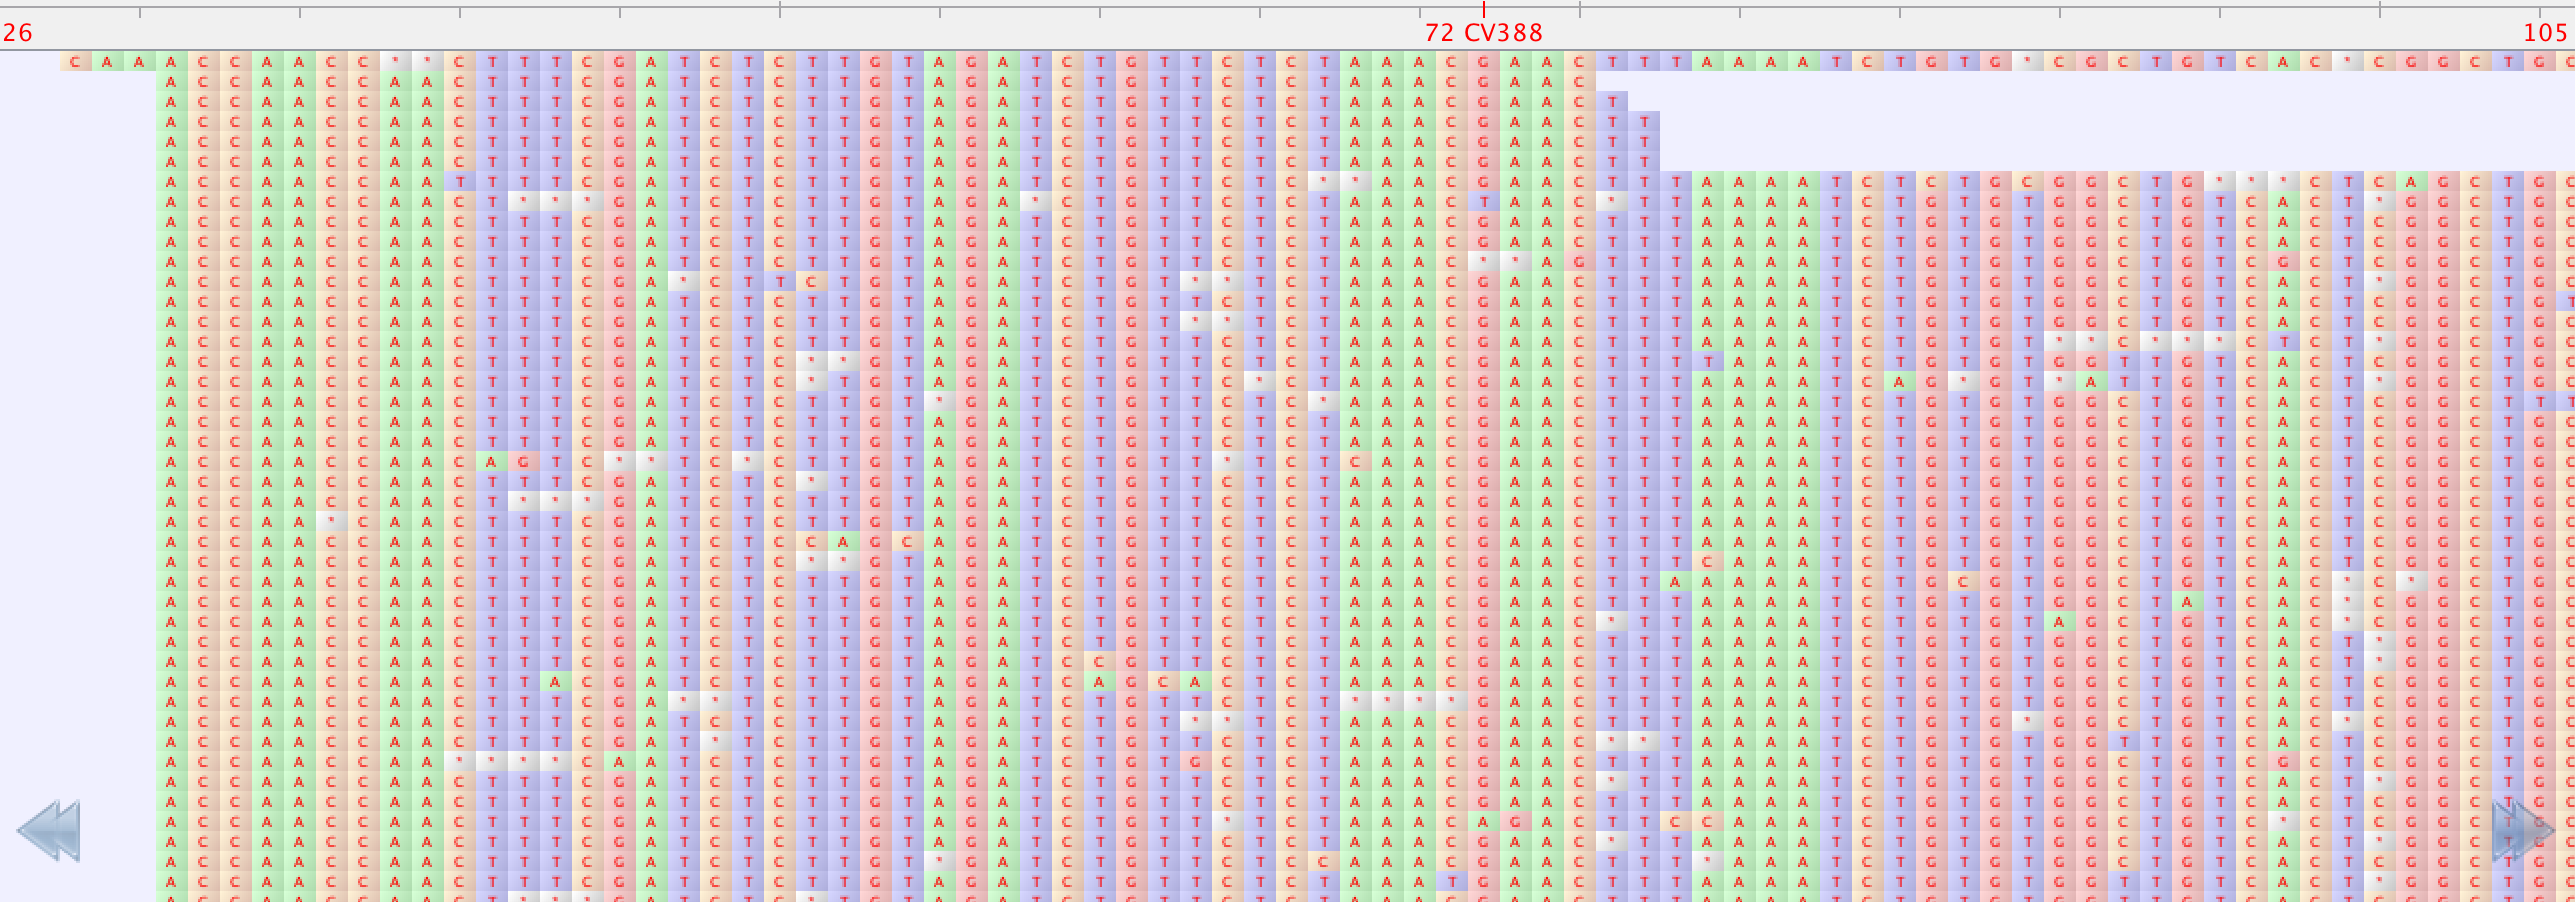
\includegraphics[width=0.99\textwidth]{../ms/figs/sam-tablet.png}
\caption{\textbf{SAM file graphical representation.} The software Tablet \comment{ref } was used. Each base call is colour coded so that base calls that disagree with the consesnsu are obvious. The 72th nucleotide in this alignment has a coverage of 388 reads.}
\label{fig:sam}
\end{figure}

The nucleotide-level probabilistic sequence can be constructed from this
alignment. The algorithm that we suggest is as follows.

We begin by initializing an empty \(5\times\ell\) matrix \(\nps'\). Each
label in Figure \ref{fig:sam} has an associated probability score. These
labels denote a row in \(\nps\), and their location on the genome
denotes the columns, say (\(\sq{A}, j\)). At this entry, we add the
corresponding quality score to whatever was there before.

By this construction, the sum of each column represents the coverage at
that location. Dividing each entry of \(\nps'\) by the sum of that
column results in \(\nps\). For our proposed propagation methods, it is
convenient to work with \(\nps'\) until probabilities are necessary.

It is important to note that many NGS platforms use paired reads where
the same genome is read in both directions. In these situations, the two
reads are not independent and should not be treated as such. Our
implementation involves taking the average of the qualtiy scores. If the
quality scores were 90\% \(\sq{A}\) for one read and 95\% \(\sq{A}\) in
the second read, then 0.925 is added to the \(\sq{A}\) row in \(\nps'\).
If the two reads were 60\% \(\sq{A}\) and 55\% \(\sq{C}\) in the two
reads, then the average of 0.6 and 0 wold be added to the \(\sq{A}\) row
and the average of 0 and 0.55 would be added to the \(\sq{C}\) row. This
is equivalent to simply dividing the quality scores by 2 if they are
paired. This is advantageous as it allows us to parallelize the reading
of SAM files without needing to know which read it is paired with.

\hypertarget{consensus-sequence-fastq-files}{%
\subsubsection{Consensus sequence FASTQ
files}\label{consensus-sequence-fastq-files}}

For most published genome sequences, the short read files are not
available. It is common to find the so-called consensus sequence, which
is the sequence that represents the most commonly called base at each
location, along with a single quality score for each location. The
methods for obtaining Phred scores when converting a SAM file to a
consensus FASTQ differ by software
\citep[\citet{keithSimulatedAnnealingAlgorithm2002},
\citet{liMappingShortDNA2008}]{liAdjustQualityScores2004}, but generally
involve a computation that includes all of the Phred scores of the bases
that agree with the consensus (\eg if the short reads have \sq{A} with
Phred of 30, \sq{A} with a Phred of 31, and \sq{C} with phred of 15,
then the Phred scores of 30 and 31 are combined in software-defined way,
usually incorporating extra information on top of the Phred score).

As a first simplifying step, we ignore insertions and deletions. Given a
base call and its associated quality score at each position, we can
assume that the other bases are all equally likely with probability
\(\epsilon/3\). For example, let's assume the output sequence after
fragment sequencing and alignment is \sq{ACATG} and its associated
quality scores are respectively \(Q=60,30,50,10,40\). The probabilistic
sequence is: \begin{equation}
S = 
\begin{pmatrix}
1-10^{-6} & 10^{-3}/3  & 1-10^{-5} & 10^{-1}/3 & 10^{-4}/3  \\
10^{-6}/3 & 1-10^{-3}  & 10^{-5}/3 & 10^{-1}/3 & 10^{-4}/3  \\
10^{-6}/3 & 10^{-3}/3  & 10^{-5}/3 & 10^{-1}/3 & 1-10^{-4} \\
10^{-6}/3 & 10^{-3}/3  & 10^{-5}/3 & 1-10^{-1} & 10^{-4}/3\\
0&0&0&0&0 \\
\end{pmatrix}
\end{equation}

Usually, the genetic sequence \sq{ACATG} would be considered as certain
and quality scores discarded. In contrast, within the probabilistic
sequence framework the probability the sequence is \sq{ACATG} is only
0.899
\({\displaystyle(=(1-10^{-6})\times (1-10^{-3})\times (1-10^{-5})\times (1-10^{-1})\times (1-10^{-4}))}\).

Insertions and deletions (``indels'\,') can be included in the uniform
framework. Here, we propose that the nucleotides probabilities are
defined conditional on an indel but other models are possible. For a
given position, the error probability is \(\epsilon = 10^{-Q/10}\)
(\(Q\) is the quality score) and we assume the probability a deletion
happens at this position is \(d\). Conditional on not being deleted, the
probability to have the base called is \((1-d)(1-\epsilon)\) and the
other three nucleotides can occur with probability \((1-d)\epsilon/3\).
Hence, if we assume the base call is \sq{A}, the column of the \nlps for
that position is \begin{equation}
\begin{pmatrix}
(1-d)(1-\epsilon)  \\
(1-d)\,\epsilon / 3  \\
(1-d)\,\epsilon / 3  \\
(1-d)\,\epsilon / 3  \\
d\\
\end{pmatrix}
\label{eq:deletion}
\end{equation}

\hypertarget{consensus-sequence-fasta-files}{%
\subsubsection{Consensus sequence FASTA
files}\label{consensus-sequence-fasta-files}}

\begin{itemize}
\tightlist
\item
  Analysis will not draw any firm conclusions, but\ldots{}

  \begin{itemize}
  \tightlist
  \item
    stress testing for your analysis, e.g.~could resample genomes at
    different overall error rates, then simulate error rates from
    overall rate at each location, then see how much it F's up your
    analysis.
  \end{itemize}
\end{itemize}

In the absense of any measured uncertainty we are constrained with what
we can do. Any uncertainty that we impose upon the data will be a
principled assumption. However, imposing our assumptions can still be
very useful as a ``stress test'' of our analysis; we can assume
different levels/types of uncertainty and quantify the stability of our
results.

The error probability at any given nucleotide location can be simulated
as a beta distribution, i.e.~

\[
\epsilon_j \sim\text{Beta}(\alpha, \beta)
\]

The called base at position \(j\) will be assigned \(1- \epsilon\) as
the probability, then the remaining bases (not includeing a gap) will be
assigned \(\epsilon_j/3\). To incorporate gaps, another probability
\(d\) can be generated as the ``gap probability''. With these defiend,
the nucleotide-level uncertainty sequence at the \(j\)th column
(supposing the base call at location \(j\) was \(\sq{A}\)) can be
generated as:

\[
\nps = 
\bordermatrix{
&\scriptscriptstyle{j}  \cr
\sq{A} & (1 - d/4)(1-\epsilon_j) \cr
\sq{C} & (1 - d/4)\epsilon_j/3 \cr
\sq{G} & (1 - d/4)\epsilon_j/3 \cr
\sq{T} & (1 - d/4)\epsilon_j/3 \cr
\sq{-} & d \cr
}
\]

This uncertainty sequence is completely fabricated, but downstream
analyses can be evaluated by choosing values of \(\alpha\), \(\beta\),
and \(d\) based on previous studies and propagating these uncertainties
into downstream analysis.

\hypertarget{propagation-of-uncertainty-via-resampling}{%
\subsection{Propagation of uncertainty via
resampling}\label{propagation-of-uncertainty-via-resampling}}

\begin{itemize}
\tightlist
\item
  Works in any analysis
\item
  provides something like bootstrapped variance or an extra prior
  sampling step
\end{itemize}

The most general way to propagate uncertainty is through resampling.
Given \(\nps\) and assuming that locations are independent (or
pre-defining biologically-reasonable sequences and calculating their
probabilities), uncertainty can be propagated by re-sampling the
sequences according to their probability and re-running the analysis on
each set of sampled sequences (I don't have a citation for this, but I
believe Peter Piper sampled a set of sampled sequences).

Re-sampling can either be done simply based on the nucleotide-level
uncertainty as a multinomial distribution. If the \(j\)th column of
\(\nps\) is (0.5, 0.2,0.2,0.09.0.01), then we could sample \(\sq{A}\)
with 50\% probability, \(\sq{C}\) with 20\%, etc. However, this
disregards the coverage at each location, thereby disregarding the
variance of the error probabilities.

To incorporate the variance of the errors, a Dirichlet-Multinomial
sampling scheme can be derived by assuming that the error probabilities
follow a Dirichlet prior and the bases follow a multinomial likelihood.
For each base at each location, the entry for \(\nps'\) is defined as
the sum of the probabilities (one minus the error probabilities). Thes
values can be used as the parameters in the Dirichlet prior, from which
base probabilities can be sampled.

For example, if the \(j\)th column of \(\nps'\) is (1200.45, 200.09,
100.74, 121.11, 0), then possible base probabilities could be (0.743,
0.126, 0.062, 0.070, 0), (0.739, 0.121, 0.066, 0.074, 0), or (0.744,
0.128, 0.056, 0.071, 0). In contrast, if the \(j\)th column of \(\nps'\)
were (12.4, 1.2, 0.4, 1.7, 0), then some samples from the Dirichlet
distribution might be (0.759, 0.059, 0.029, 0.153, 0), (0.916, 0.065,
0.009, 0.009, 0), or (0.779, 0.117, 0, 0.104, 0). The lower coverage is
incorporated into the analysis by the increase in the variance of the
Dirichlet distribution.

In a maximum likelihood framework, this is similar to bootstrapping. In
fact, the ultimate effect of this would be to decrease the bootstrap
confidence to a level that is more in line with the actual uncertainty
in the data.

In a Bayesian framework, this could be incorporated as prior
distribution on each nucleotide. For large collections of large
sequences, this increases the dimensionality dramatically. In the next
section, we provide a proposal for reducing the number of sequences that
must be sampled.

\hypertarget{reducing-computational-burden-with-sequence-level-uncertainty}{%
\subsection{Reducing computational burden with sequence-level
uncertainty}\label{reducing-computational-burden-with-sequence-level-uncertainty}}

Suppose we wish to use a single sequence to estimate some parameter
\(\theta\) (for instance, the p-value for whether a sequence is a
particular variant or the lineage assignment for grafting to a
pre-computed tree) and we are interested in the effect that uncertainty
has on this estimate. Computational burden can be partially alleviated
by incorporating sequence-level uncertainty.

To start with, a cut-off probability can be set for the nucleotide
uncertainty. Any base that has a 1/1000 error rate (its entry in
\(\nps\) is larger than 99.9\%) can be set to a 0\% error rate. With
this change, the sequence uncertainty for all possible sequences (or all
bioligically feasible sequences) can be calculated. Label these
uncertainties \(a_i\).

The sequences can be ordered according to their uncertainty, with the
most likely sequence having uncertainty \(a_{(1)}\), the second-most
likely sequence \(a_{(i)}\), etc. The analysis can be performed using
the most likely sequence, resulting in an estimate \(\theta_{(1)}\). The
analysis can be re-run with the second-most likely sequence,
\(\theta_{(2)}\). Given just these two estimates, a weighted estimate of
\(\theta\) given the 2 most likely sequences could be found as:

\[
\hat\theta_{(2)} \approx \theta_{(1)} \tilde a_{(1)} + \theta_{(2)}\tilde a_{(2)}\text{, where }\tilde a_{(j)}=a_{(j)}/\sum_{i=1}^2a_{(i)}
\]

The third-most likely sequence can be analysed, resulting in
\(\hat\theta_{(3)}\). This process can be repeated until new estimates
do not have any impact on the results (conversion criteria could be set,
but a graphical representation of \(\theta_{(i)}\) would be more
informative). If convergence is not clearly met, the cut-off can be
reduced until enough sequences are obtained.

With this algorithm, the computational burden is separated into
calculating the sequence liklihood for the most likely sequences and
running the analysis enough times to be confident convergence is
acheived.

For analyses that require a set of sequences, the likelihoods for the
set of sequences can be calculated as the product of the likelihoods
(or, for computational stability, the sum of the log-likelihoods) of the
individual sequences. The algorithm above can be adjusted accordingly.

\hypertarget{applications}{%
\section{Applications}\label{applications}}

\hypertarget{hiv}{%
\subsection{HIV}\label{hiv}}

\emph{Copy from David, re-word as necessary.}

\hypertarget{sars-cov-2}{%
\subsection{SARS-CoV-2}\label{sars-cov-2}}

In this section, we demonstrate the re-sampling method on lineage
assignment of SARS-CoV-2. Sequences are sampled from \(\nps'\) and then
assigned a lineage based on the current state-of-the-art in phylogenetic
analyis.

\hypertarget{pangolearn}{%
\subsubsection{PangoLEARN}\label{pangolearn}}

We use the lineage designations described in
\citet{rambautDynamicNomenclatureProposal2020} and assign our sequences
to lineages using the pangoLEARN tool (pangolin version 2.3.2,
pangoLEARN version 2021-02-21) that the authors have made available
(\url{github.com/cov-lineages/pangolin}). This tool uses a decision tree
model to determine which lineage a given sequence is most likely to
belong to. The tool also reports a bootstrap support probability as a
measurement of the tool's confidence in its assignment. We demonstrate
that even the best available tools are underestimating the variance and
therefore producing overconfident conclusions.

\hypertarget{data}{%
\subsubsection{Data}\label{data}}

The data for this application were downloaded from NCBI's SRA web
interface (\url{https://www.ncbi.nlm.nih.gov/sra/?term=txid2697049}).
Search results were filtered to only include runs that had SAM files. To
select which runs to download, a selection of 5-10 files from each of 20
non-sequential results pages were chosen. Once collecting the run
accession numbers from the search results, an R script was run to
download the relevant files and check that all information was complete.
23 out of 300 files were labelled incomplete due to having too few reads
(possibly because the download timed out) or not containing a CIGAR
string. The GISAID accession numbers for the seqeunces we used are
provided in the appendix.

There was no particular reason for choosing any given file, but the
resulting data should not be viewed as a random sample. Each result page
likely includes several runs from the same study, and runs were chosen
arbitrarily within each result page. We were not attempting a completely
random sampling strategy, we simply wanted a collection of runs on which
to demonstrate our methods.

\hypertarget{re-sampling-the-call-probability-matrix}{%
\subsubsection{Re-sampling the call probability
matrix}\label{re-sampling-the-call-probability-matrix}}

Since pangoLEARN is a pre-trained model, the analysis is not
computationally burdensome. Sampling 10,000 different sequences from a
call probability matrix is reasonable, even on a mid-range consumer
laptop.

For this analysis we use the most basic resampling strategy. We simply
draw probabilities from the Dirichlet distribution with parameters
defined by \(\nps'\), sample base calls from the multinomial
distribution, then use pangoLEARN to determine the lineage assignment.

Locations with 0 reads were discarded. This is a somewhat arbitrary
choice since random draws from the Dirichlet distribution when the sum
of the parameters (which, in this case, corresponds to the coverage) is
small are essentially draws from the uniform distribution.

In \ref{fig:covidcalls}, each row represents resamples from one SAM
file. Each bar represents one lineage assignment from pangolin. The
width of the bars represents the sum of the weights (genome likelihoods)
of sampled sequences. Bars are subdivided to visualize these weights.

\begin{figure}
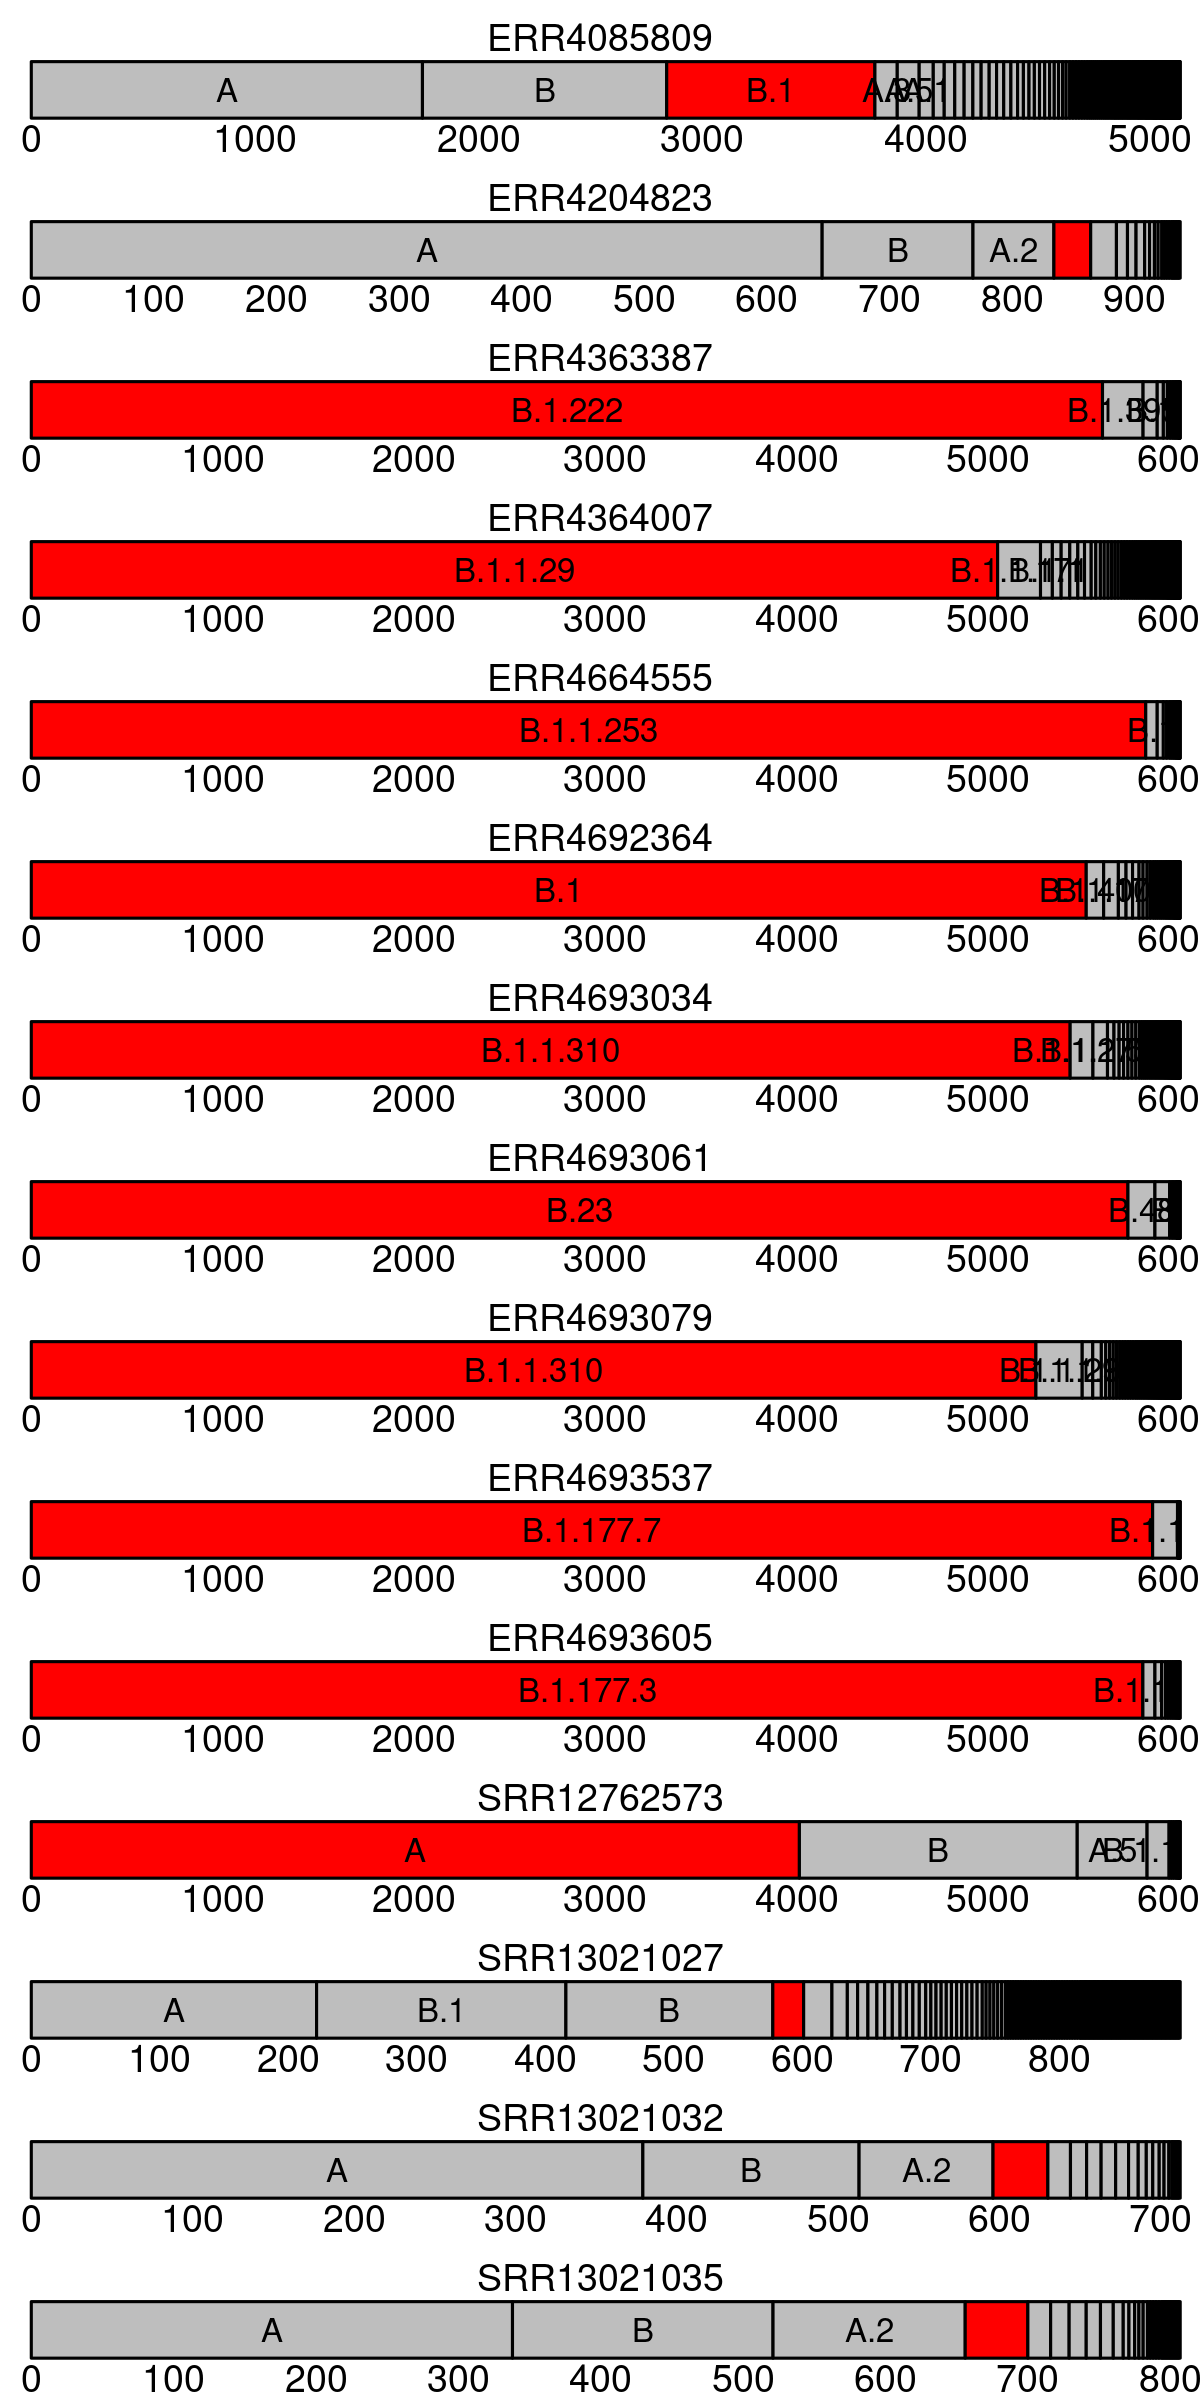
\includegraphics[width = 0.47\textwidth]{../figures/stacked-lineages.png}
\label{fig:covidcalls}
\caption{Distribution of called lineages from pangolin. Red bars indicate the lineage of the most probable sequence.}
\end{figure}

Initial analyses used pangolin version 2.0.8, which used multinomial
logistic regression, rather than decision trees, to assign lineages.
This procedure resulted in bootstrap support values that varied from 0.6
to 1. After upgrading to pangolin version 2.3.2, which uses a decision
tree model, all bootstrap probabilities are reported as 1.

\hypertarget{sequential-re-analysis-with-genome-likelihoods}{%
\subsubsection{Sequential re-analysis with genome
likelihoods}\label{sequential-re-analysis-with-genome-likelihoods}}

If the purpose is to investigate how robust a given analysis is to the
uncertainty in the genome, a more direct approach than sampling can be
taken.

\hypertarget{conclusions}{%
\section{Conclusions}\label{conclusions}}

\hypertarget{for-pangolin}{%
\subsection{For Pangolin}\label{for-pangolin}}

\hypertarget{for-phylogenetics-in-general}{%
\subsection{For phylogenetics in
general}\label{for-phylogenetics-in-general}}

\hypertarget{for-analysis-of-genetic-data}{%
\subsection{For analysis of genetic
data}\label{for-analysis-of-genetic-data}}

\begin{itemize}
\tightlist
\item
  Our method does not preclude tertiary analyses to test for systematic
  errors or deviations from a Mendelian inheritance pattern assumption.
\item
  Our method allows for adjustments for Phred or more sophisticated
  genome likelihoods.
\end{itemize}

\clearpage

\hypertarget{appendix-traversing-the-sequence-likelihoods}{%
\section{Appendix: Traversing the Sequence
Likelihoods}\label{appendix-traversing-the-sequence-likelihoods}}

We shall denote \(\mathbf M\) as the matrix containing the largest and
second largest call probabilities in each column of \(\nps\) (\ie, the
probabilities of the two most probable base calls). \(\mathbf M\) has
the same number of columns as \(\nps\), but only two rows. For LMP-3,
this would include the top three probabilities.

The most probable sequence is the one corresponding to the product of
the first row of \(\mathbf M\). We'll denote this probability as \(P_0\)

The second most probable sequence is found by choosing the lowest entry
in the first row of \(\mathbf M\) and substituting that base with the
second most probable base. We denote this substitution as a set
\(I_1=\{j\}\), such that the probability of the second most probable
sequence is:

\[
P_1 = \left(\prod_{i\in \overline I_1}\mathbf M_{(1, i)}\right)\left(\mathbf M_{(2, j)}\right)
\]

\noindent where \(\overline I\) denotes the complement of \(I\) (all
locations \emph{not} in \(I\)) and \(\mathbf M_{(1, j)}\) denotes the
first row and \(j\)th column of \(\mathbf M\).

Determining the third most probable sequence requires a comparison. It
is not clear whether keeping the substitution in the previous step and
choosing the next lowest most probable base will result in a larger
likelihood than reverting the substitution in the previous step and
choosing a new location to substitute.

Suppose the second lowest entry in the first row of \(\mathbf M\) is at
column \(k\). Our decision for calculating \(P_2\) involves choosing
between the sets of locations \(I_{2-1}\cup \{k\} = \{j, k\}\) versus
\(\left(I_{2-1}\setminus\{j\}\right)\cup\{k\} = \{k\}\), where
\(I_{2-1}\) represents the set of substitutions in the previous step. We
should choose the set that maximizes the likelihood, leaving us to test
the following condition:

\begin{align}
\left(\prod_{i\in \overline {\{j,k\}}}\mathbf M_{(1, i)}\right)\left(\mathbf M_{(2, j)}\mathbf M_{(2, k)}\right) &\stackrel{?}{>} \left(\prod_{i\in \overline {\{k\}}}\mathbf M_{(1, i)}\right)\left(\mathbf M_{(2, k)}\right) \\
\Leftrightarrow \mathbf M_{(2, j)} &\stackrel{?}{>} 1
\end{align}

  \bibliography{supbib.bib}

\end{document}
